\documentclass{beamer}

\usepackage{listings}
\usepackage{graphicx}
\usepackage{mathtools}
\usepackage{tikz}

\usetikzlibrary{matrix,chains,scopes,fit}

\begin{document}
    \title{Demystifying Haskell}
    \subtitle{An in-depth examination of the Fibonacci sequence.}
    \author{Andrew Rademacher}

    \definecolor{dkgreen}{rgb}{0,0.6,0}
    \definecolor{gray}{rgb}{0.5,0.5,0.5}
    \definecolor{mauve}{rgb}{0.58,0,0.82}

    \lstdefinelanguage{JavaScript}{
        keywords={typeof, new, true, false, catch, function, return, null, catch, switch, var, if, in, while, do, else, case, break},
        keywordstyle=\color{blue}\bfseries,
        ndkeywords={class, export, boolean, throw, implements, import, this},
        ndkeywordstyle=\color{darkgray}\bfseries,
        identifierstyle=\color{black},
        sensitive=false,
        comment=[l]{//},
        morecomment=[s]{/*}{*/},
        commentstyle=\color{purple}\ttfamily,
        stringstyle=\color{red}\ttfamily,
        morestring=[b]',
        morestring=[b]"
    }

    \lstset{frame=tb,
        language=JavaScript,
        aboveskip=3mm,
        belowskip=3mm,
        showstringspaces=false,
        columns=flexible,
        basicstyle={\small\ttfamily},
        numbers=none,
        numberstyle=\tiny\color{gray},
        keywordstyle=\color{blue},
        commentstyle=\color{dkgreen},
        stringstyle=\color{mauve},
        breaklines=true,
        breakatwhitespace=true
        tabsize=3
    }

% FRAME:TITLE
    \frame{\titlepage}

% FRAME:FIBONACCI
    \begin{frame}
        \frametitle{The Fibonacci Sequence}

        \begin{columns}[c]
            \begin{column}[T]{5cm}
                \begin{itemize}
                    \item Sequence is infinite
                    \item Sequence is self-referencing
                    \item Values grow exponentially
                    \item Values are always positive
                \end{itemize}
            \end{column}
            \begin{column}[T]{5cm}
                \begin{figure}
                    \centering
                    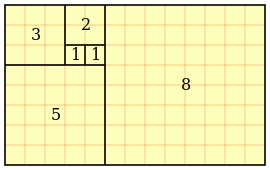
\includegraphics[height=3cm]{./fibs/images/FibonacciBlocks.png}
                \end{figure}

                \begin{figure}
                    \centering
                    \begin{math}
                        \left\{1,1,2,3,5,8...\right\}
                    \end{math}
                \end{figure}
               
                \begin{figure}
                    \centering
                    \begin{math}
                        F_{n} = F_{n-1} + F_{n-2}
                    \end{math}
                \end{figure}
            \end{column}
        \end{columns}
    \end{frame}

% FRAME:JAVASCRIPT
    \lstset{language=JavaScript}
    \begin{frame}[fragile=singleslide]
        \frametitle{Traditional JavaScript Implementation}

        \begin{lstlisting}
        function getFibs (n) {
            var fibs = [1, 1];
            for (var i = 2; i <= n; i++) 
                fibs.push(fibs[fibs.length - 1] + fibs[fibs.length - 2]);

            return fibs;
        }
        \end{lstlisting}
    \end{frame}

% FRAME:JAVA
    \lstset{language=Java}
    \begin{frame}[fragile=singleslide]
        \frametitle{Traditional Java Implementation}
        
        \begin{lstlisting}
        public static BigInteger[] getFibs(int n) {
            BigInteger[] fibs = new BigInteger[n + 1];
            fibs[0] = BigInteger.valueOf(1);
            fibs[1] = BigInteger.valueOf(1);
            for (int i = 2; i <= n; i++)
                fibs[i] = fibs[i - 1].add(fibs[i - 2]);

            return fibs;
        }
        \end{lstlisting}
    \end{frame}

% FRAME:PROCESS
    \begin{frame}[fragile=singleslide]
        \frametitle{Imperative Process}

        \sffamily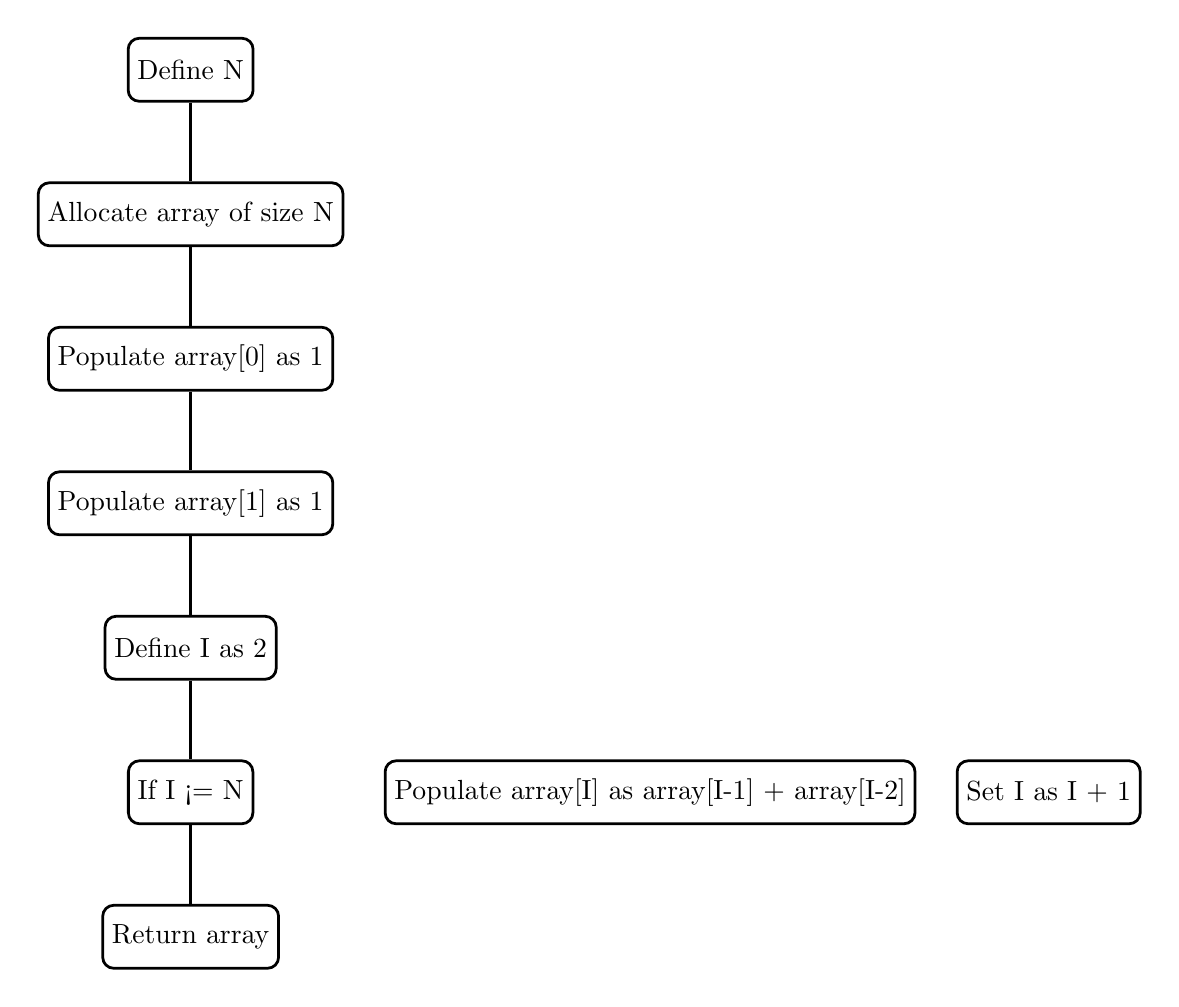
\begin{tikzpicture}
            \matrix (m) [
                matrix of nodes,
                column sep=5mm,
                row sep=1cm,
                nodes={
                    draw,
                    line width=1pt,
                    anchor=center,
                    text centered,
                    rounded corners,
                    minimum width=1.5cm, minimum height=8mm
                },
                nodes in empty cells
            ] {
                Define N \\
                Allocate array of size N \\
                Populate array[0] as 1 \\
                Populate array[1] as 1 \\
                Define I as 2 \\
                If I <= N   &   Populate array[I] as array[I-1] + array[I-2]    &   Set I as I + 1 \\
                Return array \\
            };

            { [start chain,every on chain/.style={join}, every join/.style={line width=1pt}]
                \chainin (m-1-1);
                \chainin (m-2-1);
                \chainin (m-3-1);
                \chainin (m-4-1);
                \chainin (m-5-1);
                \chainin (m-6-1);
                \chainin (m-7-1);
            };

            \tikzset{blue dotted/.style={draw=blue!50!white, line width=1pt,
                                         dash pattern=on 1pt off 4pt on 6pt off 4pt,
                                         inner sep=4mm, rectangle, rounded corners}};

        \end{tikzpicture}
    \end{frame}

% FRAME:HASKELL
    \lstset{language=Haskell}
    \begin{frame}[fragile=singleslide]
        \frametitle{New Fangled Haskell Implementation}

        \begin{lstlisting}
        fibs = 1 : 1 : [ a + b | (a, b) <- zip fibs (tail fibs) ]
        \end{lstlisting}
    \end{frame}
\end{document}
